\documentclass{beamer}

% Beamer style
%\usetheme[secheader]{Madrid}
\usetheme{CambridgeUS}
\usecolortheme[rgb={0.65,0.15,0.25}]{structure}
%\usefonttheme[onlymath]{serif}
\beamertemplatenavigationsymbolsempty
%\AtBeginSubsection

% Packages
%\usepackage[french]{babel}
\usepackage[latin1]{inputenc}
\usepackage{color}
\usepackage{dsfont, stmaryrd}
\usepackage{amsmath, amsfonts, amssymb}
\usepackage{stmaryrd}
\usepackage{epsfig}
\usepackage{/home/robin/LATEX/Biblio/astats}
%\usepackage[all]{xy}
\usepackage{graphicx}

% Commands
\definecolor{darkred}{rgb}{0.65,0.15,0.25}
\definecolor{darkgreen}{rgb}{0,0.4,0}
\newcommand{\emphase}[1]{\textcolor{darkred}{#1}}
%\newcommand{\emphase}[1]{\textcolor{black}{#1}}
\newcommand{\paragraph}[1]{\textcolor{darkred}{#1}}
\newcommand{\refer}[1]{\textcolor{blue}{[\cite{#1}]}}
\newcommand{\Refer}[1]{\textcolor{blue}{[#1]}}
\newcommand{\newblock}{}

% Symbols
\newcommand{\Bcal}{\mathcal{B}}
\newcommand{\dd}{\text{d}}
\newcommand{\Esp}{\mathbb{E}}
\newcommand{\Kbf}{{\bf K}}
\newcommand{\Gcal}{\mathcal{G}}
\newcommand{\Gam}{\mathcal{G}\text{am}}
\newcommand{\Ibb}{\mathbb{I}}
\newcommand{\Var}{\mathbb{V}}
\newcommand{\Fcal}{\mathcal{F}}
\newcommand{\Hcal}{\mathcal{H}}
\newcommand{\Lcal}{\mathcal{L}}
\newcommand{\Mcal}{\mathcal{M}}
\newcommand{\Ncal}{\mathcal{N}}
\newcommand{\Nbf}{{\bf N}}
\newcommand{\Nm}{N(\mbf)}
\newcommand{\Ocal}{\mathcal{O}}
\newcommand{\Obf}{{\bf 0}}
\newcommand{\Omegas}{\underset{s}{\Omega}}
\newcommand{\Ybf}{{\bf Y}}
\newcommand{\Pcal}{\mathcal{P}}
\newcommand{\Qcal}{\mathcal{Q}}
\newcommand{\Rbb}{\mathbb{R}}
\newcommand{\Rcal}{\mathcal{R}}
\newcommand{\sbf}{{\bf s}}
\newcommand{\Sbf}{{\bf S}}
\newcommand{\Scal}{\mathcal{S}}
\newcommand{\Ucal}{\mathcal{U}}
\newcommand{\Vcal}{\mathcal{V}}
\newcommand{\cst}{\text{cst}}
\newcommand{\ra}{\emphase{$\rightarrow$~}}

\newcommand{\fignet}{/home/robin/RECHERCHE/RESEAUX/EXPOSES/FIGURES/}

%====================================================================
\title[Exact (Bayesian) change point inference]{Exact (Bayesian) inference for change point models \\ Application to genomics}

\author[S. Robin]{S. Robin \\  }

\institute[AgroParisTech / INRA]{
  {\normalsize \begin{tabular}{rl}
    joint works with & E. Lebarbier, G. Rigaill \\
    & A. Cleynen \\
    & M. Delattre, C. L�vy-Leduc, T. Mary-Huard
    \end{tabular}} \\

  \bigskip
 \begin{tabular}{ccccc}
    
\includegraphics[width=.2\textwidth]{../FIGURES/LogoINRA-Couleur} & 
    \hspace{.02\textwidth} &
    
\includegraphics[width=.3\textwidth]{../FIGURES/logagroptechsolo} & 
    \hspace{.02\textwidth} &
    
\includegraphics[width=.2\textwidth]{../FIGURES/logo-ssb} \\ 
  \end{tabular} \\
  \bigskip 
  }

  \date[Cambridge, 2014]{\footnotesize{Inference for Change Point and Related Processes\\ Isaac Newton Institute for Mathematical Sciences, Cambridge, 3-Feb-2014}}

%====================================================================

%====================================================================
%====================================================================
\begin{document}
%====================================================================
%====================================================================

%====================================================================
\frame{\titlepage
  }

%====================================================================
\frame{\frametitle{Outline} 
  \tableofcontents
  }

%====================================================================
%====================================================================
\section[Change point problems in genomics]{Change point problems in genomics: Main issues}
%====================================================================
\frame{\frametitle{Change point problems in genomics: Main issues} 

  \paragraph{Genomic data:} often collected 'along the genome', similarly to time series
  
  \bigskip \bigskip
  \paragraph{Genomic experiments:} often aim at finding regions in which some specific event occurs:
  \begin{itemize}
   \item copy number variations (gain or loss of genomic regions)
   \item gene detection (detection of transcribed region)
   \item protein-DNA interactions (e.g. detection of protein biding sites)
   \item ...
  \end{itemize}

  \bigskip \medskip
  \paragraph{Genomic technologies} now provide information at the nucleotide resolution
  }

%====================================================================
\frame{\frametitle{Different experiments and technologies} 

  \begin{tabular}{l}
    \vspace{-.05\textheight}
    \paragraph{Comparative genomic hypridization:} microarrays / copy number variation \\
    \begin{tabular}{c}
	 \begin{overprint}
	   \onslide<1>
	   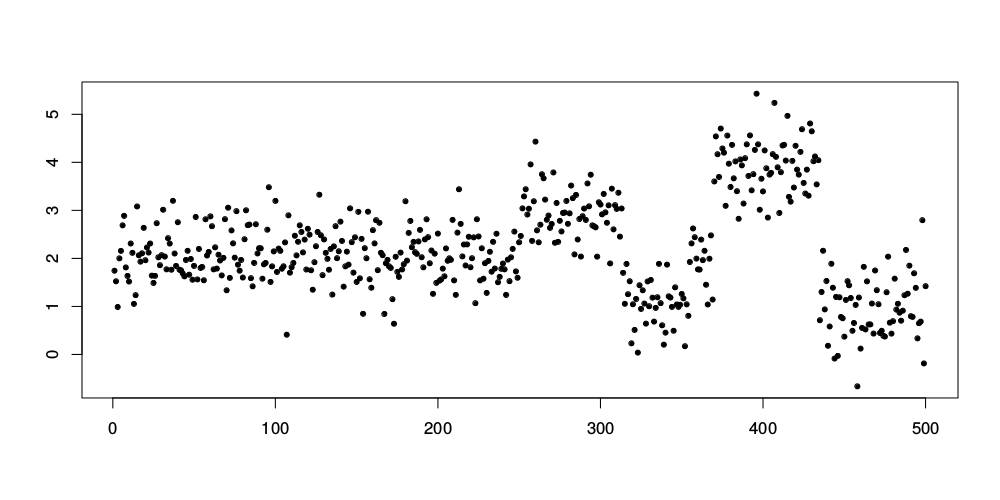
\includegraphics[height=.45\textheight, width=.9\textwidth]{../FIGURES/FigSeg-Cambridge-CGH}
	   \onslide<2>
	   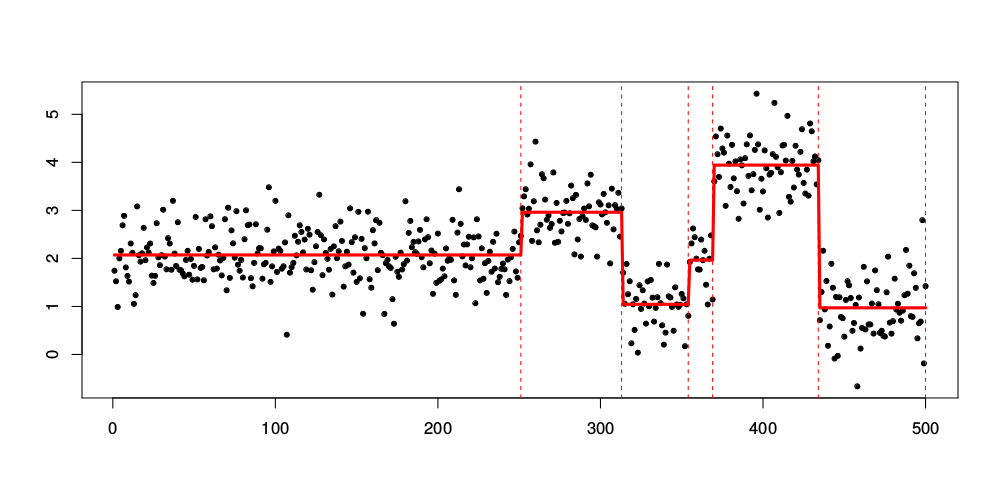
\includegraphics[height=.45\textheight, width=.9\textwidth]{../FIGURES/FigSeg-Cambridge-CGH-seg}
	 \end{overprint}
    \end{tabular}
    \\
    \vspace{-.05\textheight}
    \paragraph{RNA-sequencing:} massive sequencing / gene expression \\
    \begin{tabular}{c}
	 \begin{overprint}
	   \onslide<1>
	   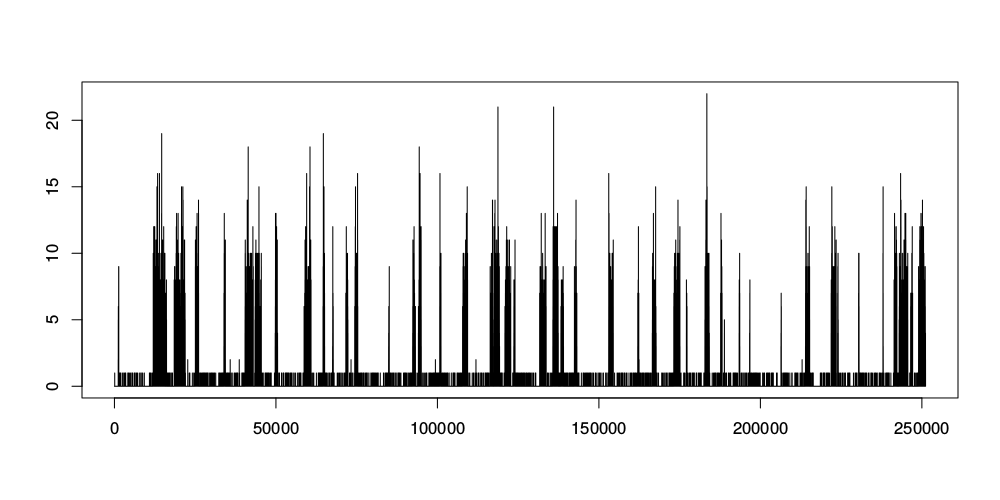
\includegraphics[height=.45\textheight, width=.9\textwidth]{../FIGURES/FigSeg-Cambridge-RNAseq}
	   \onslide<2>
	   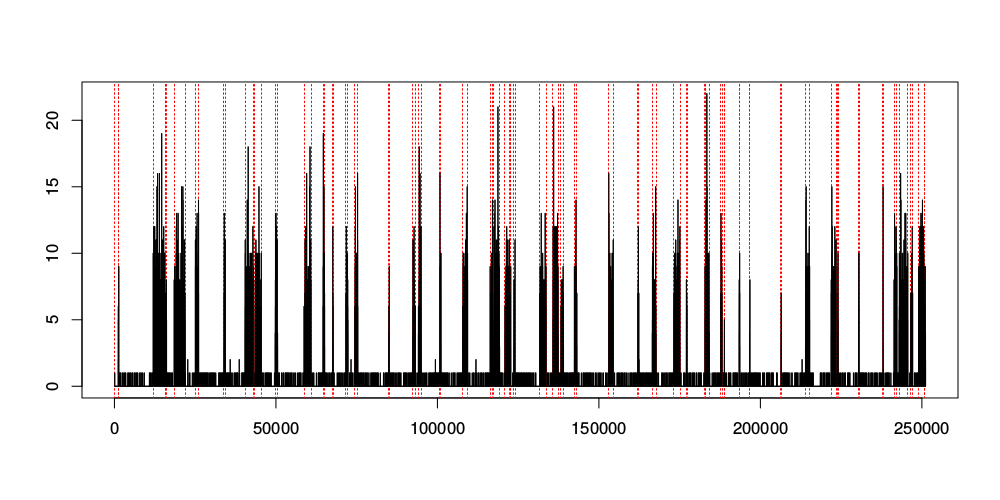
\includegraphics[height=.45\textheight, width=.9\textwidth]{../FIGURES/FigSeg-Cambridge-RNAseq-seg}
    \end{overprint}
    \end{tabular}
  \end{tabular}
  }

%====================================================================
\frame{\frametitle{Three main issues} 

  \paragraph{Modelling}
  \begin{itemize}
   \item Which distribution: Gaussian, Poisson, negative Binomial?
   \item Independence?
  \end{itemize}
  
  \bigskip 
  \paragraph{Algorithmics:} $\binom{n-1}{K-1} \approx \left(\frac{n}{k}\right)^k$ possible segmentations of $n$ points into $K$ segments
  \begin{description}
  \item[\ra] Dynamic programming retrieves the optimal segmentation in $O(Kn^2)$ for additive loss functions
  \end{description}
  
  
  \bigskip 
  \paragraph{Model selection:} How many segments: $K = $ ?
  \begin{description}
   \item[\ra] Because of discontinuity, standard model selection criteria (AIC, BIC) do not apply
  \end{description}

  }

%====================================================================
\frame{\frametitle{Two scales} 

  \paragraph{Global scale: $n \approx 10^6 - 10^8$} (whole genome) \\
  Aim = find the 'best' segmentation, not much more.
  \begin{itemize}
   \item Need for efficient algorithms (not quadratic!) \\
   \ra P. Fearnhead's \refer{KFE12} and G. Rigaill's \refer{Rig10} talk on January 16th
   \item Need for a dedicated criterion to choose $K$: see \refer{ClL13}\\
   $+$ D. Siegmund's talk on January 13th  \refer{ZhS07} 
  \end{itemize}

  \bigskip \bigskip 
  \paragraph{Local scale: $n \approx 10^3$} (genomic region) \\
  Aim = answer to more precise questions
  \begin{itemize}
   \item Reliability of the 'best' segmentation
   \item Confidence intervals for the change points
   \item Change point comparison
  \end{itemize}
  }


%====================================================================
\frame{\frametitle{Global scale: comparative study for SNP arrays}

  \paragraph{Benchmark of manually annotated profiles:} ROC curves \refer{Hoc12}
  $$
  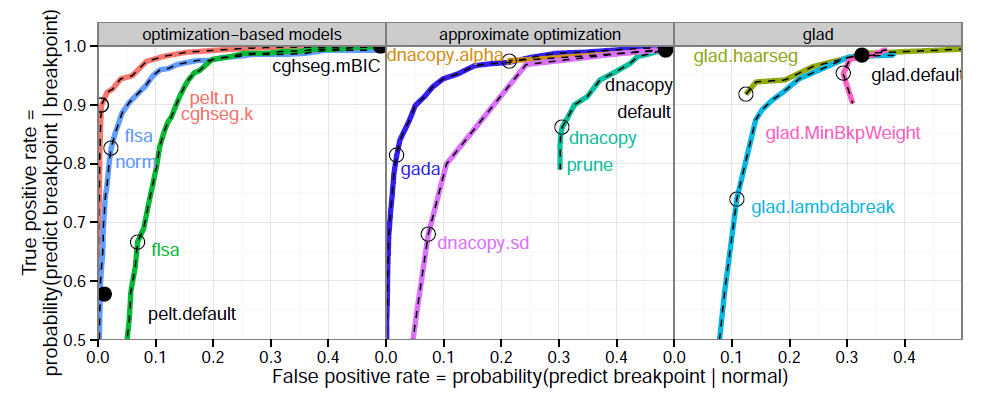
\includegraphics[width=\textwidth]{../FIGURES/Hoc12-Fig3-3}     
  $$
%   \begin{itemize}
%    \item 'Exact' methods (PDPA \refer{Rig10} and PELT \refer{KFE12}) perform best 
%    \item Model selection remains an issue.
%   \end{itemize}

 }

%====================================================================
%====================================================================
\section{Exact posterior distributions in change point models}
%====================================================================
\frame{\frametitle{Exact posterior distribution in change point models \refer{RLR11}} 
  }

%====================================================================
\frame{\frametitle{Bayesian framework for one series} 

  \paragraph{Number of segments:}
  $$
  K \sim p(K)
  $$ 

  \medskip
  \paragraph{Segmentation:}
  $$
  m = (\tau_k)_k \sim p(m|K)
  $$
  \ra Change points: $1 = \tau_0 < \dots < \tau_{K-1} < \tau_K = n +1$ \\
  \ra Segment:  $r \in m: r = \llbracket \tau_{k-1}, \tau_k \llbracket$

  \bigskip
  \paragraph{Parameters:}
  $$
  \theta = (\theta_r)_{r \in m} \sim p(\theta |m)
  $$

  \medskip
  \paragraph{Data:}
  $$
  Y = (Y_t)_{1 \leq t \leq n} \sim p(Y | \theta, m)
  $$


%   \begin{tabular}{lll}
%     Number of segments: & $K$ & $p(K)$ \\
%     ~ \\
%     Segmentation: & $m = (\tau_k)_k$ & $p(m|K)$ \\
%     (change points: & $0 < \tau_1 < \dots < \tau_{K-1} < n$) & \\
%     ~ \\
%     Segmentation space: & $\Mcal_K = \Mcal_K(\llbracket 1, n+1 \llbracket)$ & \\
%     ~ \\
%     Segment: & $r = \llbracket \tau_{k-1}, \tau_k \llbracket$ & \\
%     ~ \\
%     Parameters: & $\theta = (\theta_r)_{r \in m}$ & $p(\theta |m)$ \\
%     (segments: & $r = \llbracket \tau_{k-1}, \tau_k \llbracket$) & \\
% 
%     ~ \\
%     Data: & $Y = (Y_t)_{1 \leq t \leq n}$ & $p(Y | \theta, m)$ \\
%   \end{tabular}

  }

%====================================================================
\frame{\frametitle{Standard change point model} 

  \begin{tabular}{cc}
    \hspace{-.5cm}
    \begin{tabular}{p{.5\textwidth}}
      \onslide+<1->{\paragraph{Hierarchical model.} 
        \begin{itemize}
        \item \onslide+<2->{$K \sim p(K)$ \\~}
        \item \onslide+<3->{$m = (\tau_k)_k \sim p(m|K)$\\~}
        \item \onslide+<4->{$\theta = (\theta_r)_{r \in m} \sim p(\theta |m)$\\~}
        \item \onslide+<5->{$Y = (Y_t)_{1 \leq t \leq n} \sim p(Y | \theta, m)$}
        \end{itemize}}
    \end{tabular}
    & 
    \hspace{-1cm}
    \begin{tabular}{c}
%       \onslide+<2->{
%         \hspace{-6cm}
%         \onslide+<3->{if $t \in \textcolor{blue}{r_k}$,} \quad $Y_t$
%         \onslide+<5->{$\sim
%           \Fcal($}\onslide+<4->{$\textcolor{red}{\theta_k}$}\onslide+<5->{$)$}
%         \\}
      \begin{overprint}
        \onslide<2>
        \includegraphics[width=.5\textwidth]{../FIGURES/FigSeg-Budapest-1} 
        \onslide<3>
        \includegraphics[width=.5\textwidth]{../FIGURES/FigSeg-Budapest-2} 
        \onslide<4>
        \includegraphics[width=.5\textwidth]{../FIGURES/FigSeg-Budapest-3} 
        \onslide<5>
        \includegraphics[width=.5\textwidth]{../FIGURES/FigSeg-Budapest-4} 
        \onslide<6->
        \includegraphics[width=.5\textwidth]{../FIGURES/FigSeg-Budapest-0} 
      \end{overprint}
    \end{tabular}
  \end{tabular}

  \onslide+<6->{
  $$
  \text{\emphase{Aim:} \qquad } p(K, m, \theta | Y)
  $$
  } 
  }

%====================================================================
\frame{\frametitle{Some distributions of interest} 

  %Infer several quantities based on the observed series $Y$.
  \begin{itemize}
   \item Number of change points: 
   $$
   p(K | Y)
   $$
   \item Change point location: 
   $$
   P\{\tau_k = t | Y\} \quad \text{or} \quad P\{\tau_k = t | Y, K\}
   $$
   \item Existence of a change point: 
   $$
   P\{\exists k: \tau_k = t | Y\}
   $$
   \item Reliability of the 'best' segmentation: 
   $$
   p(\widehat{m} | Y) \quad \text{or} \quad  p(\widehat{m} | Y, K)
   $$
   \item Mean of the parameter at a given location: 
   $$
   \Esp(\theta_t | Y)
   $$
  \end{itemize}
  }
  
  
%====================================================================
\frame{\frametitle{Factorability assumptions} 

  %We require that prior distribution satisfy the following.
  
   \begin{itemize}
   \item Segmentation:
   $$
   p(m|K) = \prod_{r \in m} f(r) 
   $$
   \ra $p(m|K) = 1 \left/ |\Mcal_K| \right.$ or $p(m|K) \propto \prod_{r \in m} n_r$ \\ ~
  \item Parameter:
  $$
  p(\theta|m) = \prod_{r \in m} f(\theta_r)
  $$
  \ra independent parameters in each segment (\emphase{no homoscedasticity}) \\ ~
  \item Data:
  $$
  p(Y | m, \theta) = \prod_{r \in m} f(Y^r, \theta_r) 
  $$
  \ra data are independent from one segment to another %(but not necessarily within each segment)
   \end{itemize}
}

%====================================================================
\frame{\frametitle{Need for integrals and sums} 

  \paragraph{Model selection:} $p(K | Y) \propto p(Y | K) p(K)$
  $$
  p(Y|K) = \sum_{m \in \Mcal_K} \prod_{r\in m} \int p(Y^r|\theta_r) p(\theta_r)
  \dd \theta_r = \sum_{m \in \Mcal_K} \prod_{r\in m} p(Y^r)
  $$
  $p(Y^r)$ has a close-form when using conjugate priors

  \bigskip \bigskip 
  \paragraph{Localisation of the $k$-th breakpoint:}
  \begin{eqnarray*}
    P\{\tau_k = t | K, Y\} & \propto & \left(\sum_{m \in \Mcal_k(1, t)} \prod_{r
    \in m} p(Y^r)\right) \left(\sum_{m \in \Mcal_{K-k}(t+1, n)} \prod_{r
    \in m} p(Y^r)\right)
  \end{eqnarray*}
  
  \bigskip 
  \ra Need to sum up over the whole segmentation space $\Mcal_K$.
  }

%====================================================================
\frame{ \frametitle{Computing sums of products}

To compute
  $$
  \sum_{m \in \Mcal_K(1, t)} \prod_{r \in m} f(r),
  $$
  define the upper triangular $(n+1) \times (n+1)$ matrix $A$:
  $$
  A_{ij} = f(\llbracket i, j \llbracket ), \qquad 1 \leq i < j \leq n+1
  $$
  then
  $$
  \sum_{m \in \Mcal_K(1,t)} \prod_{r \in m} f(r) = [A^k]_{1,t+1}
  $$
  \ra all terms ($1 \leq k \leq K$, $1 \leq t \leq n+1$) are computed in {$O(K n^2)$}.  
  
  \bigskip \bigskip
  \paragraph{NB:} Similar to the shortest path dynamic programing algorithm, replacing {'max'} with {'sum'} and {'sum'} with {'product'}
  }

%====================================================================
\frame{ \frametitle{A CGH profile: $K = 3, 4$}
 
 \vspace{-.25cm}
  \begin{tabular}{lll}
    \hspace{-0.5cm}
    \begin{tabular}{p{0.25\textwidth}} 
    %Optimal segmentation
    $\widehat{m}_K =$ \\
    $\arg\max_m p(m | Y ,K)$ 
    \end{tabular}
    &
    \hspace{-0.5cm}
    \begin{tabular}{c}
      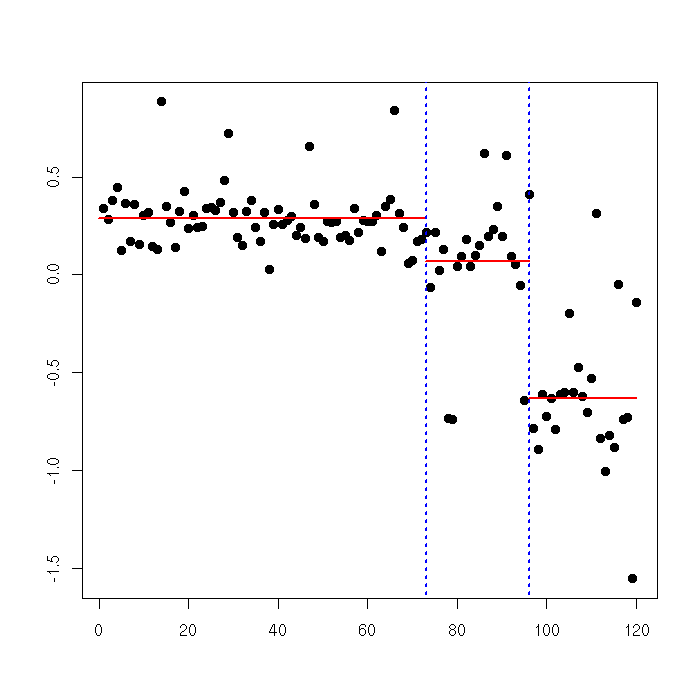
\includegraphics[width=0.3\textwidth, height=0.3\textheight,
      clip=]{../FIGURES/CopyNumberChr10_BIC}   
    \end{tabular}
    &
    \hspace{-0.5cm}
    \begin{tabular}{c}
      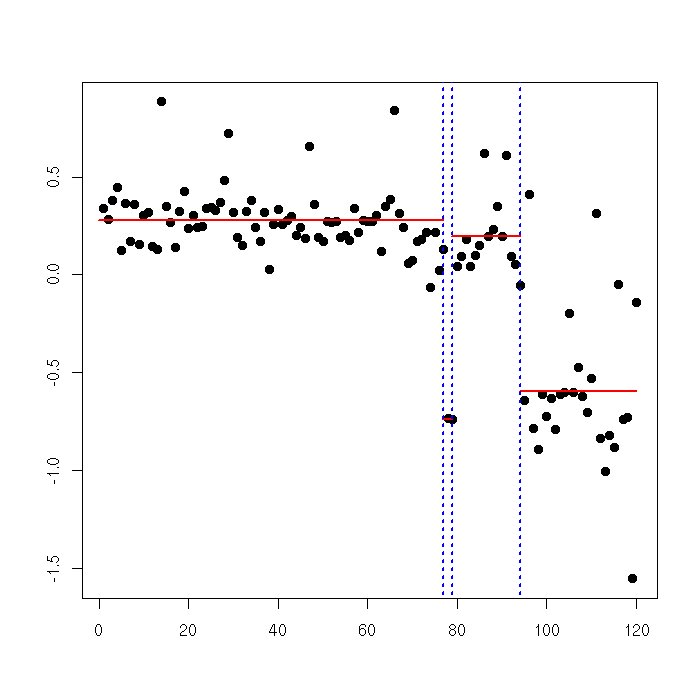
\includegraphics[width=0.3\textwidth, height=0.3\textheight,
      clip=]{../FIGURES/CopyNumberChr10_ICL}  
    \end{tabular}\\ 
    \hspace{-0.5cm}
    \begin{tabular}{p{0.25\textwidth}} 
    %Breakpoint position 
    $P\{\tau_K = t | Y, K\}$
    \end{tabular}
    &
    \hspace{-0.5cm}
    \begin{tabular}{c}
      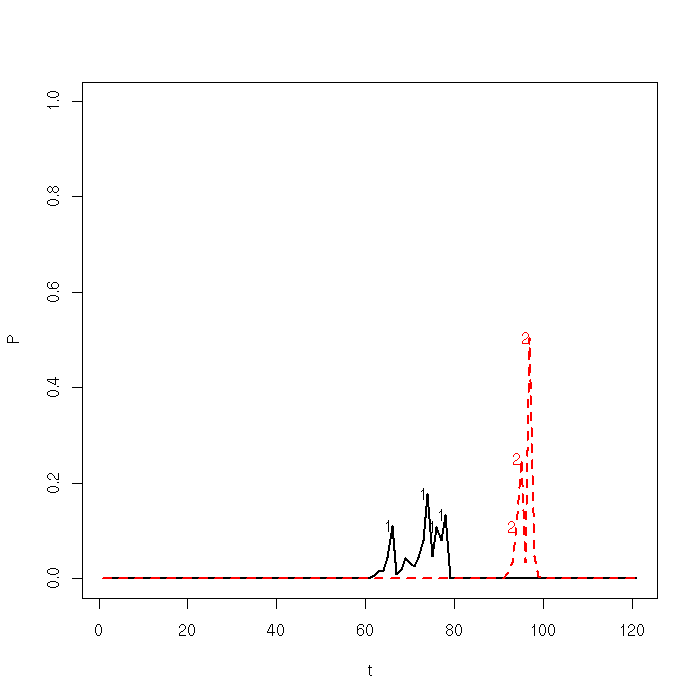
\includegraphics[width=0.3\textwidth, height=0.3\textheight,
      clip=]{../FIGURES/CopyNumberChr10_ProbaBIC}   
    \end{tabular}
    &
    \hspace{-0.5cm}
    \begin{tabular}{c}
      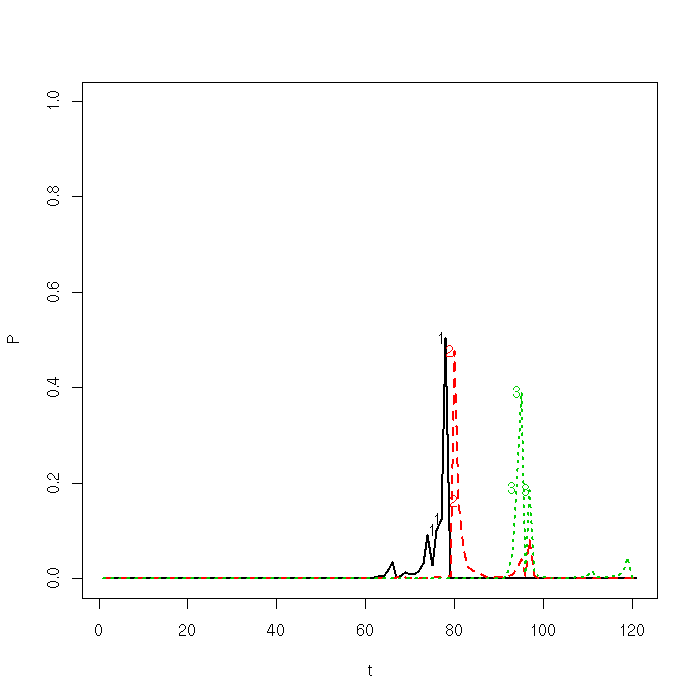
\includegraphics[width=0.3\textwidth, height=0.3\textheight,
      clip=]{../FIGURES/CopyNumberChr10_ProbaICL}  
    \end{tabular}\\ 
    \hspace{-0.5cm}
    \begin{tabular}{p{0.25\textwidth}} 
    %Segment probability 
    $P\{r \in m | Y, K\}$
    \end{tabular}
    &
    \hspace{-0.5cm}
    \begin{tabular}{c}
%      \vspace{-0cm}
      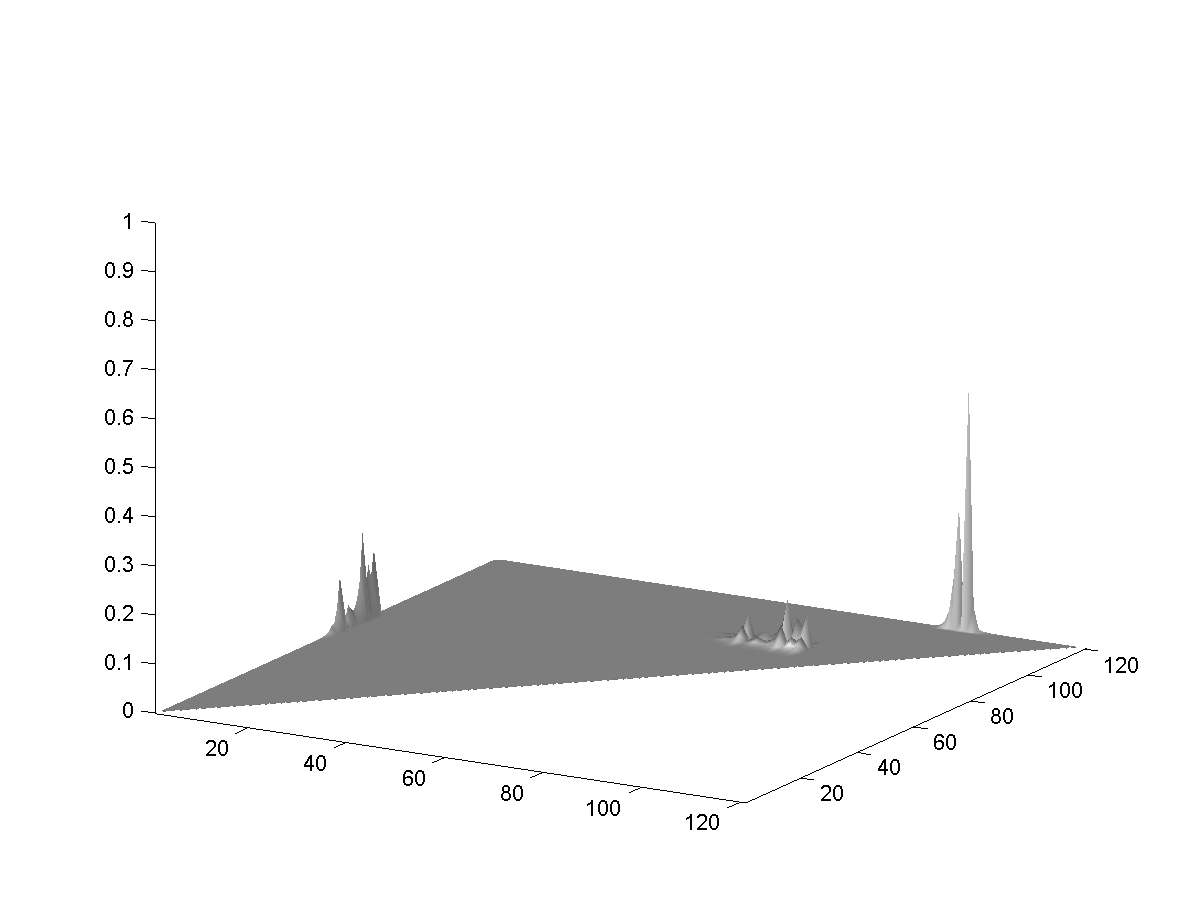
\includegraphics[width=0.32\textwidth, height=0.27\textheight,
      clip=]{../FIGURES/ProbSeg-BIC}     
    \end{tabular}
    &
%    \vspace{-.5cm}
    \begin{tabular}{c}
      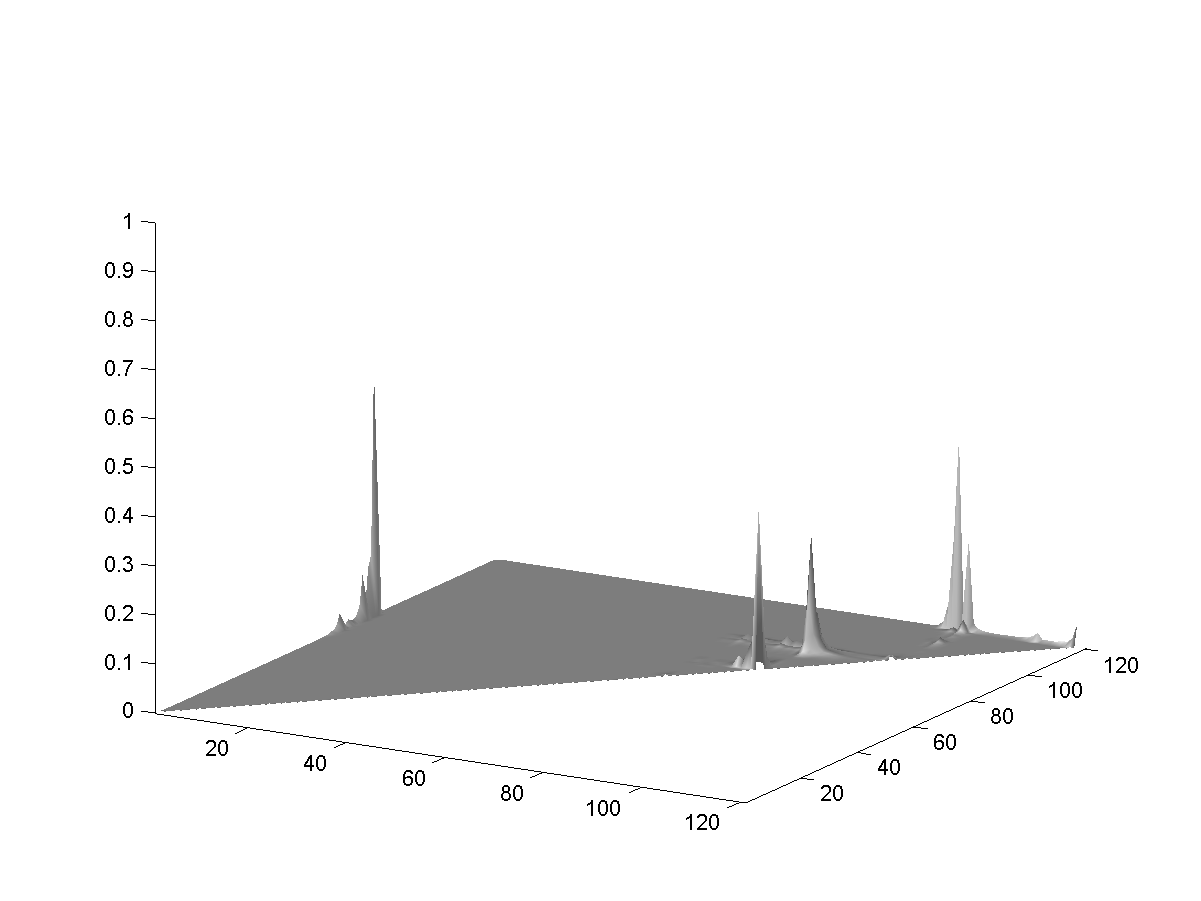
\includegraphics[width=0.32\textwidth, height=0.27\textheight,
      clip=]{../FIGURES/ProbSeg-ICL}   
    \end{tabular} 
  \end{tabular}
  }

%====================================================================
%====================================================================
\frame{ \frametitle{Model selection}

  \vspace{-.05\textwidth}
  \paragraph{Simulation:} Poisson signal alternating $\theta_0=1$ and $\theta_1$, $n = 100$. \\~

  \paragraph{Criterion} = \% of recovery of the true number of segments ($K = 5$). \\ 

  \begin{tabular}{p{.5\textwidth}p{.5\textwidth}}
    \hspace{-0.5cm}
    \begin{tabular}{p{.5\textwidth}}
	 \paragraph{Exact criteria} can be computed: \\ ~

	 $\textcolor{green}{BIC(K)} = \log p(Y, K)$ \\ ~

      $\textcolor{red}{BIC(m)} = \log p(Y, m)$ \\ ~
      
      $\textcolor{blue}{ICL(K)} = BIC(K) - H(K)$ \refer{BCG00} \\ ~\\
      $H(K) = $ entropy of $p(m | Y, K)$ 
    \end{tabular}
    &
    \hspace{-.05\textwidth}
    \vspace{-.3\textheight}
    \begin{tabular}{c}
% 	 \textcolor{green}{$BIC(K)$} \quad \textcolor{red}{$BIC(m)$} \quad
% 	 \textcolor{blue}{$ICL(K)$} \\
	 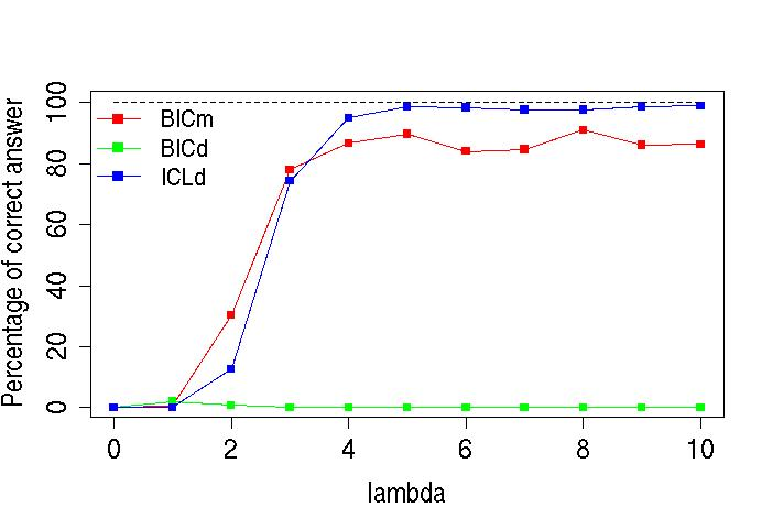
\includegraphics[width=.5\textwidth, height=.6\textheight]{../FIGURES/ICLvsBIC} \\ 
	 $\theta_1 - \theta_0, \quad \theta_0 = 1$
    \end{tabular}
  \end{tabular}
 }

%====================================================================
%====================================================================
\section{Comparing change point locations}
%====================================================================
\frame{\frametitle{Comparing change point locations  \refer{ClR13}} 
  }

%====================================================================
\frame{\frametitle{RNA-seq data} 

  \paragraph{Data:} $Y_t =$ number of reads mapped onto the genome and starting at nucleotide $t$

  $$
  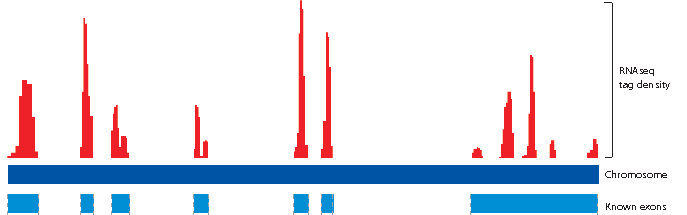
\includegraphics[width=.8\textwidth, height=.4\textheight]{../FIGURES/gb-2008-9-9-234-1}
  $$

  \Refer{genomebiology.com}

}

%====================================================================
\frame{\frametitle{Comparing transcript boundaries in yeast}

  \vspace{-.05\textheight}
  \begin{tabular}{p{.2\textwidth}p{.7\textwidth}}
    \begin{tabular}{p{.3\textwidth}}
	 One gene \\
	 \\
	 $\times$ \\
	 \\
	 Three growth \\
	 conditions: 
	 $A$, $B$, $C$
    \end{tabular}
    &
    \begin{tabular}{p{.7\textwidth}}
    \includegraphics[width=.7\textwidth]{../FIGURES/compyeastresult.pdf}
    \end{tabular}
  \end{tabular}
}

%====================================================================
\frame{\frametitle{Comparing 2 profiles}

  \paragraph{Model:} Two independent series $Y^1$ and $Y^2$

  \bigskip \bigskip
  \paragraph{Question:} Is there a shift between the two transcription starts?
  $$
  \Delta := \tau_1^1 - \tau_1^2 \overset{?}{=} 0
  $$
  
  \bigskip
  \paragraph{Posterior distribution of the shift:} 
  $$
  P\{\Delta=d|Y^1, Y^2, K^1, K^2\} 
  = \sum_t P\{\tau_ 1^1=t | Y^1, K^1\} P\{\tau_ 1^2 = t-d | Y^2, K^2\}
  $$
%   \begin{eqnarray*}
%   & & P\{\Delta=d|Y^1, Y^2, K^1, K^2\} \\
%   & & \qquad = \sum_t P\{\tau_ 1^1=t | Y^1, K^1\} P\{\tau_ 1^2 = t-d | Y^2, K^2\}   
%   \end{eqnarray*}
  
  \bigskip
  \paragraph{Application to RNAseq:}
  \begin{itemize}
  \item Consensus distribution: negative Binomial ${\mathcal NB}(\theta_r, \phi)$ 
  \item $\phi$ is first estimated using a robust moment-based estimator \refer{JKK92} (no common parameter allowed...)
  \item Exact posterior 95\% credibility intervals can then be derived
  \end{itemize}
 
}

%====================================================================
\frame{\frametitle{Back to the example}

  3 comparisons ($A/B$, $A/C$, $B/C$) $\times$ 4 change points:
  
\centerline{\includegraphics[width=.8\textwidth, height=.8\textheight]{../FIGURES/cred-yeast.pdf}}

}

%====================================================================
\frame{\frametitle{Comparing $I > 2$ profiles}

  \vspace{-0.5cm}
  \begin{tabular}{cc}
    \hspace{-0.5cm}
    \begin{tabular}{p{.6\textwidth}}
      \paragraph{Event of interest:} consider $I$ profiles
      $$
      E_0 = \{\tau_{k_1}^1 = \dots = \tau_{k_I}^I\}
      $$

      ~\\
      \paragraph{Aim: } evaluate the posterior
      $$
      P(E_0 | {\bf Y}, {\bf K})
      $$
%       can be computed exactly in ${\mathcal O}(In^2)$.
      
	 ~\\ ~\\
	 ${\bf Y} = (Y^1, \dots Y^I)$, 
	 ${\bf K} = (K^1, \dots K^I)$, ... 
    \end{tabular}
    &
    %\hspace{-.5cm}
    \begin{tabular}{c}
       \paragraph{Graphical model:} \\ ~\\
      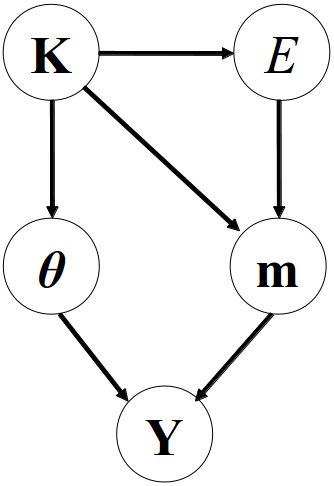
\includegraphics[width=.2\textwidth]{../FIGURES/GraphModel}
    \end{tabular}
  \end{tabular}

  }

%====================================================================
\frame{\frametitle{Boundary shifts} 

  \paragraph{Efficient summation rules} only apply for independent series or given $E_0$ \\ 
  
  \begin{enumerate}
   \item Consider the surrogate model $Q$ where series are fully independent:
  \begin{eqnarray*} 
   Q(\Ybf, E_0 | \Kbf) & = & \sum_t \prod_\ell  \left[(A_\ell)^{k_\ell}\right]_{1, t} \left[(A_\ell)^{K_\ell-k_\ell}\right]_{t+1, n+1}\\
   Q(\Ybf | \Kbf) & = & \prod_\ell \left[(A_\ell)^{K_\ell}\right]_{1, n+1}
  \end{eqnarray*}
  \item Then, via probability change,
  \begin{eqnarray*} 
  & & P(E_0 | \Ybf, \Kbf) \\
  & = & \frac{p_0}{q_0} Q(\Ybf, E_0 | \Kbf) \left/
  \left[ \frac{p_0}{q_0} Q(\Ybf, E_0 | \Kbf) +  \frac{1 - p_0}{1 - q_0} Q(\Ybf, E_1 | \Kbf) \right] \right.
  \end{eqnarray*}
  where $E_1 = \overline{E}_0$, $p_0 = P(E_0 | \Kbf)$, $q_0 = Q(E_0 | \Kbf)$%, $Q(\Ybf, E_1 | \Kbf) = Q(\Ybf | \Kbf) - Q(\Ybf, E_0 | \Kbf)$
%   and $A_\ell$ stands for the matrix $A$ as defined in (\ref{eq:matrixA}), corresponding to series $\ell$.
  \end{enumerate}

  }

%====================================================================
\frame{\frametitle{Back to the example}

$$
\begin{array}{lccccc}
& \tau_1 & \tau_2 & \tau_3 & \tau_4 \\ 
\hline \\
P(E_0(A, B) | \Ybf, \Kbf) & 0.32 & 0.30 &0.99 & 10^{-5} \\ \\
P(E_0(A, C) | \Ybf, \Kbf) & 4 \; 10^{-4} & 0.99 &0.99 & 6 \; 10^{-3} \\ \\
P(E_0(B, C) | \Ybf, \Kbf) & 5 \; 10^{-2} & 0.60 & 0.99 & 0.99 \\ \\
P(E_0(A, B, C) | \Ybf, \Kbf) & 10^{-3} & 0.99  & 0.99 & 6 \; 10^{-3} \\ 
\end{array}
$$

\bigskip
\ra Differences at the UTR's end but not at internal exon boundaries.
}

%====================================================================
\frame{\frametitle{Various isoforms in yeast?} 

  \paragraph{$P(E_0|\Ybf, \Kbf)$} for yeast genes with 2 expressed exons
  $$
  \begin{tabular}{cc}
  \includegraphics[width=.4\textwidth]{../FIGURES/statall-all} 
  & 
  \includegraphics[width=.4\textwidth]{../FIGURES/statall2} 
  \\
   $p_0 = (.5, \;.5, \;.5, \;.5)$
   &
   $p_0 = (.9, \;.99, \;.99, \;.9)$
  \end{tabular}
  $$
}

%====================================================================
%====================================================================
\section[Chromosome-chromosome interactions]{Chromosome-chromosome interactions (on-going work)}
%====================================================================
\frame{\frametitle{Chromosome-chromosome interactions (on-going work)}
  }

%====================================================================
\frame{\frametitle{Chromosome-chromosome interactions}

  \paragraph{Chromosome conformation} within the nucleus of the cell has a major impact on gene expression due to, e.g.
  \begin{itemize}
   \item accessibility for the transcriptional machinery
   \item spatial proximity and co-expression
  \end{itemize}
  
  \bigskip \bigskip
  \paragraph{Chromosome conformation capture:} 3C, 4C, 5C, HiC techniques provide a measure of physical interactions between all loci along the chromosome:
  $$
  Y_{ij} = f(\text{physical interactions between loci $i$ and $j$}), 
  \qquad1 \leq i < j, \leq n.
  $$
  
  \bigskip \bigskip
  \paragraph{Focus:} interaction between neighbor loci ('cis' interactions)
  }

%====================================================================
\frame{\frametitle{The data}

    \begin{tabular}{p{.4\textwidth}p{.5\textwidth}}
    \begin{tabular}{p{.4\textwidth}}
	 \paragraph{Human chromosome 21} \\ ~\\
	 
	\paragraph{NGS =} nucleotide resolution \\ 
    \ra window-width $w \approx 10^5$ \\
    \ra signal: $n \approx 10^3$ \\ ~\\
  
	 Domains found by \refer{DSY12}: \\
	 HMM on directionality index \\
	 \ra good concordance with external data
    \end{tabular}
    &
    \begin{tabular}{p{.5\textwidth}}
	 %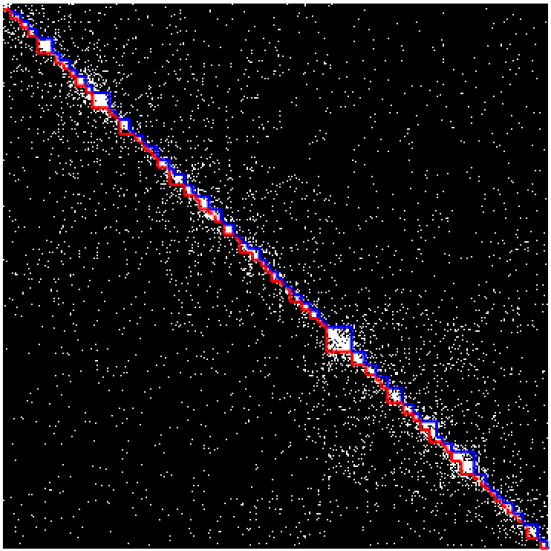
\includegraphics[height=.6\textheight]{\fignet/DLM14-JDS-Fig3}
    	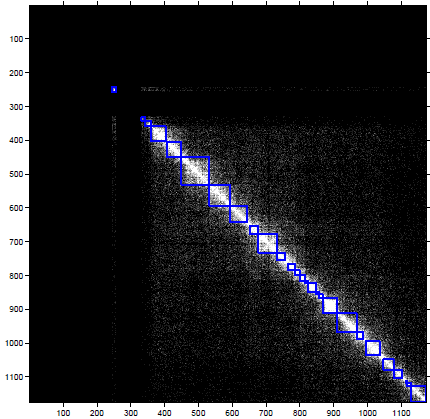
\includegraphics[width=.5\textwidth]{\fignet/DLM14-ECCB-Fig2a}
    \end{tabular}
  \end{tabular}
  }

%====================================================================
\frame{\frametitle{Block-diagonal segmentation model}

  \begin{tabular}{p{.45\textwidth}p{.5\textwidth}}
    \begin{tabular}{p{.45\textwidth}}
	 \paragraph{Cis-interactions = } blocks along the diagonal:
      \begin{itemize}
	 \item $t^*_0, \dots, t^*_K=$ change points \\ ~
	 \item $D_1, \dots, D_K = $ half-square diagonal blocks \\ ~
	 \item $E_0 = \cap_k \overline{D_k} = $ below the diagonal blocks
	 \end{itemize}
    \end{tabular}
    &
    \begin{tabular}{p{.45\textwidth}}
    	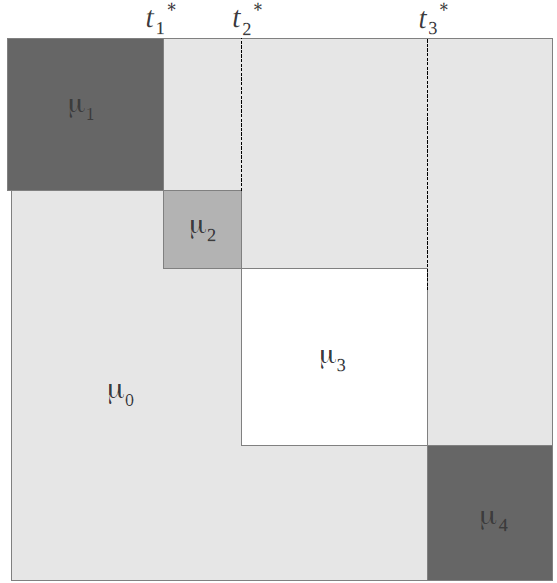
\includegraphics[width=.45\textwidth]{\fignet/DLM14-JDS-Fig1}
    \end{tabular}
  \end{tabular}
%   $$
%   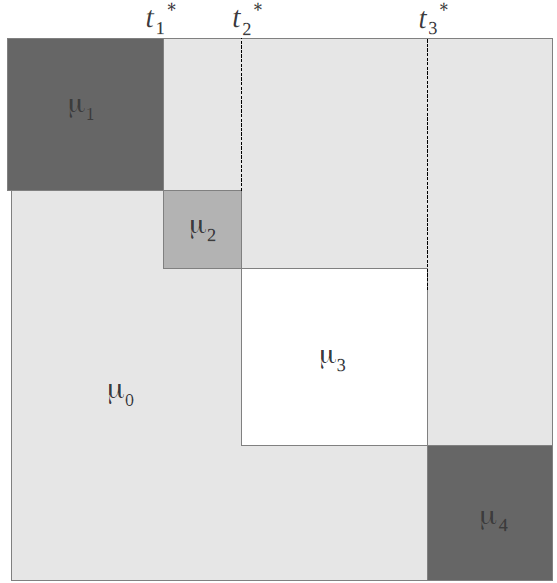
\includegraphics[height=.6\textheight]{\fignet/DLM14-JDS-Fig1}
%   $$
  }

%====================================================================
\frame{\frametitle{Model}

  \paragraph{Model:} $(Y_{ij})_{1 \leq i < j \leq n}$ independent:
  \begin{eqnarray*}
   (i, j) \in D_k: \quad Y_{ij} & \sim & p(\cdot; \mu_k) \\
   (i, j) \in E_0: \quad Y_{ij} & \sim & p(\cdot; \mu_0)
  \end{eqnarray*}
  
  \bigskip 
  \paragraph{Log-likelihood:} 
  \begin{eqnarray*}
  \log p(Y; \mu, t^*) & = & \sum_k \left(\sum_{(i, j) \in D_k} \log p(Y_{ij}; \mu_k)\right) + \sum_{(i, j) \in E_0} \log p(Y_{ij}; \mu_0) \\
   & = & \sum_k \left(\sum_{(i, j) \in D_k} \log p(Y_{ij}; \mu_k) + \sum_{(i, j) \in R_k} \log p(Y_{ij}; \mu_0)\right)
  \end{eqnarray*}
  where $R_k =$ rectangle on the left side of $D_k$
  
  }

%====================================================================
\frame{\frametitle{Inference}

  \paragraph{Maximum likelihood inference} via dynamic programming, using
  \begin{itemize}
  \item a preliminary estimate of $\mu_0$: $\widehat{\mu}_0$
  \item the cost function for segment $r = \rrbracket s, t \rrbracket$ 
  $$
  C(s, t) = \sum_{s < i < j \leq t} \log p(Y_{ij}; \widehat{\mu}_r) + \sum_{s < i \leq t} \sum_{1 < j \leq s} \log p(Y_{ij}; \widehat{\mu}_0)
  $$
  \end{itemize}
  \ra The problem resumes to a 1D segmentation problem

  
  \bigskip \bigskip
  \paragraph{Model selection:} models are not nested according to $K$ \\
  \ra the likelihood does not necessarily increase with $K$ \\
  \ra in absence of a dedicated criterion, we use
  $$
  \widehat{K} = \arg \max_K \log p_K(Y; \widehat{\mu}, \widehat{t})
  $$

  }

%====================================================================
\frame{\frametitle{On-going work}

  \begin{tabular}{p{.5\textwidth}p{.5\textwidth}}
    \begin{tabular}{p{.5\textwidth}}
	 \paragraph{Chromosome 21:} \\ ~\\
	 \begin{overprint}
	 \onslide<1>
	 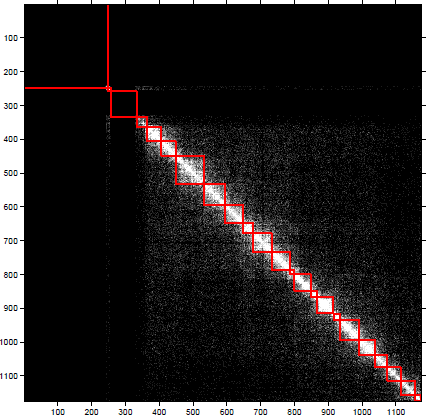
\includegraphics[width=.5\textwidth]{\fignet/DLM14-ECCB-Fig2b}
	 \onslide<2->
	 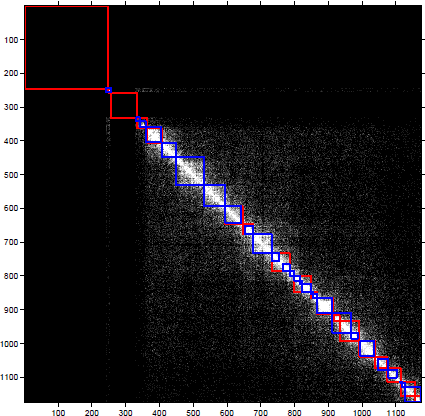
\includegraphics[width=.5\textwidth]{\fignet/DLM14-ECCB-Fig2c}
	 \end{overprint}
    \end{tabular}
    &
    \begin{tabular}{p{.5\textwidth}}
    \onslide+<3>{
	 \paragraph{To-do list:}
	 \begin{itemize}
	 \item model selection \\~
	 \item deal with original data ($n \approx 10^{6-8}$) \\~
	 \item consider trans-interactions \\~
	 \item ...
	 \end{itemize}
    }
    \end{tabular}
  \end{tabular}

    }

%====================================================================
%====================================================================
\section*{Advertisement}
%====================================================================
\frame{\frametitle{Advertisement}

  Some R packages available at {\tt cran.r-project.org}: \\~
  \begin{description}
   \item[CGHseg:] analysis of CGH and SNP  arrays for copy number variation analysis using segmentation models: one or several profiles, with/without covariates, with/without calling (Gaussian) \refer{PLH11} \\ ~
   \item[Segmentor3IsBack:] fast exact segmentation for various cost functions (Gaussian, Poisson, negative binomial) \refer{CKL13} \\ ~
   \item[EBS:] exact Bayesian segmentation, posterior probabilities of breakpoints, BIC and ICL criteria, comparison of change point location, (Gaussian, Poisson, negative binomial) \refer{ClR13}
  \end{description}

  }

%====================================================================
%====================================================================
\section*{Appendix}
%====================================================================

{\tiny
  \bibliography{/home/robin/Biblio/ARC,/home/robin/Biblio/AST,/home/robin/Biblio/SSB}
  %\bibliographystyle{/home/robin/LATEX/astats}
  \bibliographystyle{plain}
  }

%====================================================================
%====================================================================
\end{document}
%====================================================================
%====================================================================


\frame{\frametitle{}
  }

